\documentclass{standalone}
\usepackage{tkz-fct}
\usepackage{amsmath}
\usepackage{tkz-tab}
\usepackage{tkz-euclide}
\usepackage{color}
\newcommand{\vect}[1]{\overrightarrow{#1}}

\renewcommand*\familydefault{\sfdefault}
\usepackage{sansmath}
\sansmath
\definecolor{gray75}{gray}{0.75}
\begin{document}
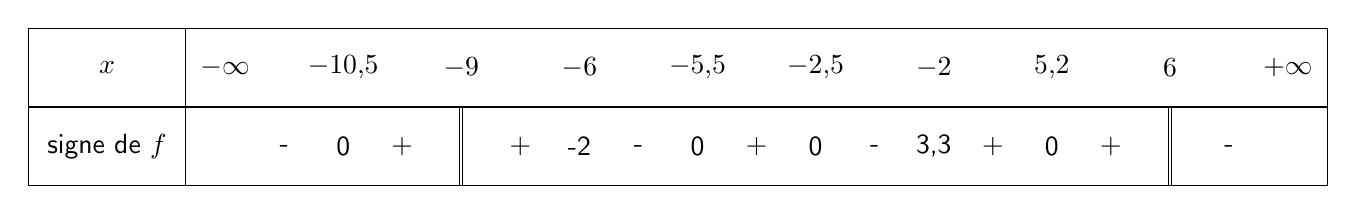
\begin{tikzpicture}
\tkzTabInit[espcl=1.5]
{$x$
/1,
signe de $f$
/1}
{$-\infty$,$-10{,}5$,$-9$,$-6$,$-5{,}5$,$-2{,}5$,$-2$,$5{,}2$,$6$,$+\infty$}
\tkzTabLine{,$-$,$0$,$+$,d,$+$,$-2$,$-$,$0$,$+$,$0$,$-$,$3{,}3$,$+$,$0$,$+$,d,$-$}

\end{tikzpicture}

\end{document}
 % Local Variables:
 % TeX-command-extra-options: "-shell-escape"
 % End: